\chapter{Estrategia de análisis}

En el capítulo anterior se describieron los conceptos básicos de
estadística necesarios para poder realizar un análisis de búsqueda
de nueva física.




En este capítulo se va a describir el el mayor
desafío del análisis desde el punto de vista estadístico: como
construir el modelo del análisis.

%% \hll{Ahora que hemos establecido una forma general para el modelo y trasladamos
%% las preguntas básicas de mediciones, descrubrimeinto y exclusión en el lenguaje
%% estadístico, estamos listos para encarar el desafío estadístico fundamental:
%% construir el modelo}

\section{Regiones de Señal, Control y Validación}
%---------------
% Signal Region
%---------------
Un análisis de física que quiera estudiar un determinado fenómeno nuevo involucra
la definición de una región en el espacio de fase, obtenida aplicando una selección
a un conjunto de observables cinemáticos, donde el modelo de señal predice un exceso
significativo de eventos sobre el nivel de fondo predicho en la misma región. A esta
región enriquecida por señal se la llama región de señal (SR).

%-----------
% Fondos/CR
%-----------
Una de las tareas mas importantes del análisis entonces sera estimar los procesos
de fondos que contaminan la región de señal. Para esto existen dos técnicas principales:
simulaciones Monte Carlo, y basandose en los datos observados.

La primera de las técnicas consiste en generar una gran cantidad de eventos utilizando técnicas
de Monte Carlo del proceso físico considerado. En general este proceso se realiza en varias etapas.
Con un generador de eventos se realiza la simulación de la interacción fuerte (por ej.
{\madgraph}). Luego con el mismo u otro generador se realiza la lluvia de partones y el
proceso de hadronizacion (por ej. {\pythia}). Y finalmente se simula la interacción de las
partículas generadas con el detector ({\geant}). A cada proceso que se simula de esta forma
lo llamaremos muestra en referencia a la muestra correspondiente generada con Monte Carlo.

Para cada proceso físico tenemos que el numero de eventos esperado por unidad de tiempo (tasa)
estará dado por:

\begin{equation}
  \text{tasa} = (\text{flujo}) \times (\text{sección eficaz}) \times (\text{eficiencia}) \times (\text{aceptancia})
\end{equation}
%
donde la sección eficaz esta predicha por la teoría, el flujo es controlado por
el acelerador, y la eficiencia y la aceptancia son propiedades del detector y los
criterios de la selección de eventos. Esta relación no es mas que la reformulacion
invariante de la probabilidad de dispersión predicha por primeros principios de la
mecánica cuántica $P(i\to f) = |\braket{i}{f}|^2/(\braket{i}{i}\braket{f}{f})$.

Si llamamos seccion eficaz efectiva $\sigma_\text{eff}$ al producto de la seccion eficaz,
la eficiencia y la aceptancia, el numero de eventos esperado para un dado proceso ($\nu$)
va a ser el producto de la luminosidad integrada en el tiempo, L y la seccion eficaz efectiva:

\begin{equation}
  \nu = L \sigma_\text{eff}
\end{equation}

Sin tener en cuenta los efectos del detector, la distribucion de un observable $x$ sera

\begin{equation}
 f(x) = \frac{1}{\sigma_\text{eff}} \frac{d\sigma_\text{eff}}{dx}
\end{equation}

Como ya hemos simulado el pasaje de las particulas por el detector podemos estimar
la distribucion subyacente $f(x)$ creando un histograma del observable $x$ con la muestra
simulada.

La validez de la simulaciones MC esta fundamentalmente relacionada a como la teoría
subyacente modela las observaciones experimentales. Las debilidades que puedan tener
la estimación de fondo a partir de las simulaciones derivan de las debilidades
de las simulaciones propiamente dichas. Por este motivo, en el caso de que haya
deficiencias en el modelado por parte de las simulaciones, existe una motivación
para utilizar métodos que puedan dar una estimación de los fondos a partir de los
datos observados. Existen distintas formas de poder estimar un fondo a partir
de los datos observados. En el Capítulo \ref{cap:fondos} se describirán las utilizadas
en este análisis.

Y existe una tercera forma para estimar los fondos, que consiste en utilizar la estimacion
proveniente de las simulaciones MC, pero corregirla con los datos. Para
esto se puede definir una o más regiones de control (CR) en las cuales el fondo dominante
pueda ser controlado comparadolo con los datos observados en esa misma región. Las CR
son diseñadas especialmente para tener una alta pureza en uno de los procesos de fondo
y deben estar libres de contaminación de señal.

A través del ajuste a los datos, el número de eventos observado en una CR es usado para
\emph{normalizar} el número de eventos estimado de fondo en todas las regiones, especialmente
en la SR. Es decir, las predicciones iniciales de las simulaciones MC son escaleadas al
nivel observado en la correspondiente CR, usando un factor de normalización calculado en
el ajuste. Este factor es utilizado entonces en la extrapolacion a las demas regiones.

%--------------------
% Validation regions
%--------------------
Otro componente importante del análisis es la validación del modelo utilizado
para predecir los fondos en las SR. Con este motivo se definen regiones de validación
(VR) que se encuentren entre las CR y las SR en términos de los principales observables
cinemáticos en los criterios de selección. El diseño de las VR es un compromiso entre
minimizar la contaminación de la señal, pero a su vez siendo efectivas en la validación
de la extrapolación entre CR y SR. En la {\fig} \ref{fig:regions_sketch} se puede ver
un esquema de las regiones descriptas anteriormente.

\begin{figure}[h]
  \centering
  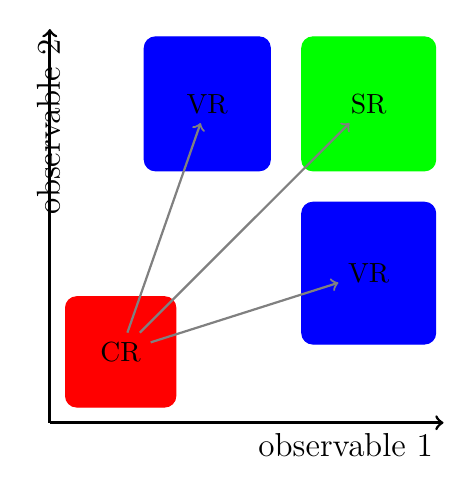
\begin{tikzpicture}

  \tikzstyle{region} = [rounded corners, fill]


  \draw[line width=1, ->] (0,0) -- (5,0) node[below left] {\large observable 1};
  \draw[line width=1, ->] (0,0) -- (0,5) node[left=0.5,rotate=90] {\large observable 2};

  \draw[region, red] (0.2,0.2) rectangle (1.6,1.6) node[midway,black] (CR) {CR};

  \draw[region, green] (3.2,3.2) rectangle (4.9,4.9) node[midway,black] (SR) {SR};

  \draw[region, blue] (3.2,1.0) rectangle (4.9,2.8) node[midway,black] (VR1) {VR};
  \draw[region, blue] (1.2,3.2) rectangle (2.8,4.9) node[midway,black] (VR2) {VR};

  \draw[->,gray, line width=0.8] (CR) -- (SR);
  \draw[->,gray, line width=0.8] (CR) -- (VR1);
  \draw[->,gray, line width=0.8] (CR) -- (VR2);

\end{tikzpicture}

  \caption{Esquema}
  \label{fig:regions_sketch}
\end{figure}

Es importante que las CR, VR y SR sean estadísticamente independientes para poder combinar
la pdf que modela cada región en una pdf conjunta. Esto es fundamental ya que al ajustar
los parámetros de la función likelihood se deberá hacer en un ajuste simultáneo. Esto es
importante para poder compartir los parámetros de los fondos y las incertezas sistemáticas
entre las distintas regiones de forma consistente.

%------------------------
% Extrapolacion CR -> SR
%------------------------
\section{Extrapolación y factores de transferencia}

Una de las suposiciones que se hizo en la sección anterior fue que las variables cinemáticas
que se usan para diferencias CR(s) y SR(s) están bien modeladas después de haber ajustado
la pdf total a los datos en las CR(s).
Una vez que los procesos de fondo dominantes son normalizados en las CR(s), las
correspondientes modificaciones en la pdf pueden ser extrapoladas a las VRs, las cuales
son utilizadas para verificar la validez de esta suposición inicial.
Una vez que se demuestra el acuerdo entre las predicciones del fondo normalizadas y los datos observados
en las VRs, las predicciones del fondo son extrapoladas a las SR(s), y comparadas con los
datos observados allí. Este proceso es llamado \emph{unblinding} y es útil para validar
la validez de las extrapolaciones y es utilizado ampliamente en fisica para tener confianza
en los metodos usados y evitar utilizar predicciones prematuraas y evitar un posible sesgo
en el resultado final.

En el procedimiento explicado anteriormente se utiliza de forma implicita los denominados
\emph{factores de transferencia}. Las predicciones de los fondo normalizadas en el ajuste son:

\begin{align}
  N_p^{\text{est}}(\text{CR}) &= \mu_p \times \text{MC}_p (\text{CR}) \\
  N_p^{\text{est}}(\text{SR}) &= \mu_p \times \text{MC}_p (\text{SR})
\end{align}
%
donde $N_p^{\text{est}}(\text{CR})$ y $N_p^{\text{est}}(\text{SR})$ es el número de eventos
estimado para cada proceso de fondo $p$ y $\text{MC}_p^{\text{est}}(\text{CR})$ y $\text{MC}_p^{\text{est}}(\text{SR})$
es el número de eventos obtenido de las simulaciones MC. El factor $\mu_p$
es el factor de normalización obtenido en el ajuste a datos.

%% En el ajuste, los valores estimados de fondo son tipicamente driven por la estadistica de las
%% CRs.

Definiendo $N_p^\text{fit}(\text{SR})$ como el valor ajustado en la CR,
podemos ecribir de forma equivalente:

\begin{align}
  N_p^\text{est}(\text{SR}) &= \mu_p \times \text{MC}_p (\text{SR}) \nonumber \\
  &\equiv N_p^\text{fit}(\text{CR}) \times \left[ \frac{\text{MC}_p(\text{SR})}{\text{MC}_p(\text{CR})} \right]
\end{align}

El cociente que aparece dentro de los corchete es llamado \emph{factor de transferencia} (TF).
Un aspecto importante de los TF es que que las incertezas sistemáticas de los
valores estimados de fondo pueden ser parcialmente cancelados en la extrapolación.
La incerteza total en el numero de eventos de fondo en la SR es por lo tanto
una combinación de las incertezas estadísticas en las CRs y la incerteza sistemática
residual de la extrapolación. Por esta razón las CR suelen definirse con una selección
un poco más relajada, para incrementar la estadística, sin aumentar significativamente
la incerteza en los TF, para reducir las incertezas en la SR.

\section{Modelo}

La función likelihood conjunta contiene el parámetro de interés (la intensidad de la señal),
los factores de normalización para los procesos de fondo, y los llamados parámetros nuisance que modelan
el impacto de las incertezas sistemáticas. Cada incerteza sistemática $i$ se describe con
un parámetro nuisance $\theta_i$ que interpola entre el valor nominal y las variaciones
de las incertezas sistemáticas. Es decir para las variaciones de las incertezas sistemáticas
$\pm \sigma$ tenemos $\theta_i = \pm 1$ y $\theta_i = 0$ para el valor nominal.

La función likelihood general $L$ es el producto de los términos de Poisson del número
de eventos en la SR y las CR, y una distribución adicional que implementa las
condiciones en las incertezas sistemáticas. Puede escribirse como:

\begin{align}
  L(\bm{n}, \bm{\theta}^0| \mu_\text{sig}, \bm{\mu}_p, \btheta) &= \mathcal{P}_\text{SR} \, \times \, \mathcal{P}_\text{CR} \, \times \, \mathcal{C}_\text{syst} \nonumber \\
  &= \Pois(n_i|\lambda_i(\mu_\text{sig}, \bm{\mu}_p, \btheta)) \, \times \, \prod_{i \in \text{CR}} \Pois(n_i|\lambda_i(\mu_\text{sig}, \bm{\mu}_p, \btheta)) \times C_\text{syst} (\btheta^0, \btheta)
\end{align}
%
Los primeros dos factores ($\mathcal{P}_\text{SR}$ y $\mathcal{P}_\text{CR}$)
reflejan las distribuciones de Poisson de $n_i$, el número de
eventos observado en cada región. El valor esperado de la distribución de Poisson
$\lambda_i$ son funciones que dependen de las predicciones de señal y los distintos fondos $p$, los
parámetros nuisance que parametrizan las incertezas sistemáticas $\btheta$, los factores
de normalización para los procesos de fondo $\bm{\mu}_p$ y también la intensidad de la
señal $\mu_\text{sig}$. Para $\mu_\text{sig} = 0$ tenemos la función likelihood para
la hipótesis de solo-fondo y con $\mu_\text{sig} = 1$ el valor esperado de señal para el
valor nominal de modelo bajo consideración.

Las incertezas sistemáticas son incluidas usando la pdf $C_\text{syst}(\btheta^0, \btheta)$,
donde $\btheta^0$ son los valores centrales de las medidas auxiliares alrededor de los
cuales $\btheta$ puede variarse al maximizar el likelihood. %\itodo{The
  %impact of changes in nuisance parameters on the expectation
  %values are described completely by the functions predicting
  %the amount of signal and background, λ S and λ i .}
Para parámetros nuisance independientes $C_\text{syst}$ es simplemente el producto
de las pdf correspondientes a las mediciones auxiliares que describen cada una de las
incertezas sistemáticas, típicamente una distribución gaussiana $G$ con ancho unidad,

\begin{equation}
  C_\text{syst} (\btheta^0, \btheta) = \prod_{j \in \text{S}} G(\theta_j^0 - \theta_j)
\end{equation}
%
donde S es el conjunto completo de las incertezas sistemáticas consideradas.
Las medidas auxiliares $\theta^0_j$ son típicamente fijadas a cero, pero pueden
variar cuando se generan los pseudo-experimentos.


%% \section{Fit}






%---
%---


%% Analyses generally rely on external predictions for the various background and signal components
%% in the data to aid the interpretation of observations, where the signal component describes the
%% process of interest. In particle physics, simulations of known and hypothesized physics processes
%% are run through a detailed detector simulation, and are subsequently reconstructed with the same
%% algorithms as the data. In addition, background samples can be constructed using data-driven
%% methods. The simulated samples may depend on one or many model parameters, for example the
%% masses of hypothesized new particles such as foreseen by supersymmetry. It may be required, for
%% instance when signals are analyzed over a multi-dimensional space of model parameters, to sample
%% from a “grid” of potential signal scenarios, with each point on that grid corresponding to a unique
%% point in the multi-dimensional parameter space. If no excess is observed in the data, exclusion
%% limits may be set within this grid, excluding a subset of the tested parameter values.

%% \itodo{Podemos pensar a un experimento de conteo en el contexto de la eq 1 con
%%   $f(x) = 1$, reduciendoce solo al termino de Poisson}


%% \section{Medidas auxiliares}

%% Las medidas auxiliares o regiones de control puede ser utilizadas para reducir
%% el efecto de las incertezas sistemáticas. Las SR o CR no son fundamentalmente
%% distintas, en este lenguaje son dos canales distintos.

%% {\bf Common example: simple counting experiment with a background}

%% Desde el punto de vista frecuentista, el fondo desconocido en la región de se\~nal es un
%% parámetro nuisance, que llamamos $\nu_B$.

%% Si el numero de eventos de se\~nal es $\nu_S$ y el numero de eventos en la región de se\~nal
%% $n_\text{SR}$, podemos escribir el modelo $\Pois (n_\text{SR}|\nu_S+\nu_B)$.

%% Como $\nu_B$ es un parámetro libre, no podemos hacer ninguna inferencia acerca de $\nu_S$.
%% En general uno tiene una estimacion del fondo, que puede venir de una muestra de control
%% con $n_\text{CR}$ eventos.
%% Si la región de control no tiene contaminación de se\~nal y esta poblado con el mismo proceso
%% de fondo que la region de se\~nal, podemos escribir $\Pois(n_\text{CR}|\tau \nu_B)$, donde $n_\text{CR}$
%% es el numero de eventos en la región de control y $\tau$ es el factor utilizado para extrapolar
%% el fondo de la región de control a la región de se\~nal\todo{o al reves?}.

%% El modelo de probabilidad total puede escribirse
%% $\vec{f}_\text{sim}(n_\text{SR}, n_\text{CR}|\nu_S,\nu_B) = \Pois (n_\text{SR}|\nu_S+\nu_B) \cdot \Pois (n_\text{CR}|\tau\nu_B)$.

%% Basados solo en la CR, se puede estimar $\nu_B = n_\text{CR}/\tau$.  Intuitivamente
%% esta estimacion viene con una ``incerteza'' de $\sqrt{n_\text{CR}}/\tau$. El punto a
%% resaltar es que podemos usar mediciones auxiliares ($n_\text{CR}$) para describir la
%% incerteza en el parámetro nuisance $\nu_B$ estadísticamente. Creamos un modelo
%% estadístico que puede tratarse con un formalismo frecuentista. Se dice que las medidas
%% auxiliares \fix{constrain} los parámetros nuisance.

%% Total probability model:

%% \begin{equation}
%%   \vec{f}_\text{tot} (\mathcal{D}_\text{sim},\mathcal{G}|\alpha) = \prod_{c \in \text{canales}} \left[ \Pois(n_c|\nu_c{(\alpha)}) \prod_{e=1}^{n_c} f_c (x_{c,e}|\alpha) \right] \cdot \prod_{p \in S} f_p (a_p|\alpha_p)
%% \end{equation}

%% \subsection{Tratamiento de las incertezas sistematicas} \label{sec:fit_syst}

%% Treatment of the Systematic Uncertainties in the likelihood is described below. Gaussian PDFs are used
%% to model the systematic uncertainties, each having nominal values $\mu^{0}$ around which $\mu$ can be varied when
%% maximizing the likelihood. Theoretical and uncertainties on the background are taken into account as
%% well as detector uncertainties on the signal. Correlations between nuisance parameters can be treated
%% properly as 1) overall scale factors fully correlated across the different regions and the different components
%% (like luminosity), 2) scale factors fully correlated across the different regions but independent per component
%% (like theory uncertainties), and 3) fully uncorrelated variables (like Monte-Carlo statistical
%% errors) with one parameter per region. %The numbers of the uncertainties used as the fit inputs can be found in \Tab \ref{}.



%% \section{Herramientas para el análisis estadístico}

%% Para el analisis estadistico se utilizo el software \texttt{HistFitter} \cite{histfitter}
%% desarrollado dentro del grupo de SUSY en ATLAS, que es una interfaz para herramientas
%% como \texttt{RooFit}, \texttt{RooStats}\cite{Moneta:2010pm} y \texttt{HistFactory}
%% \cite{Cranmer:1456844} y ademas posee una serie de scripts que facilitan el analisis cuando este
%% es muy complejo.
